\documentclass[10pt]{article}
\usepackage{amsmath} % assumes amsmath package installed
\usepackage{amsfonts,mathrsfs}
\usepackage{amssymb}
\usepackage{color}
\usepackage{graphicx}
\usepackage{epsfig}
\usepackage{epstopdf}
%\usepackage{subfigure}
\usepackage{enumerate}
\usepackage{algorithm,algorithmicx}
\usepackage{algpseudocode}
\usepackage{subcaption}

%\usepackage[]{algorithm2e}

\def\bbbr{{\rm I\!R}}
%\input{macros.tex}
%\input{slide_macros.tex}

\newtheorem{definitiox	n}{Definition}{\it}{}
\newtheorem{example}{Example}{\it}{}
\newtheorem{corollary}{Corollary}{\it}{}
\newtheorem{proposition}{Proposition}{\it}{}
\newtheorem{lemma}{Lemma}{\it}{}
\newtheorem{theorem}{Theorem}{\it}{}
\newtheorem{remark}{Remark}{\it}{}
\newtheorem{assumption}{Assumption}{\it}{}
\newenvironment{proof}[1][Proof]{\noindent\textbf{#1.} }{\ \rule{0.5em}{0.5em}}
%\newcommand{\proof}{\vspace{1mm}\noindent{\it Proof.}\quad}
%\def\qed{\quad{$\square$}} 

\textwidth=6.3in
\textheight 9in 
\setlength{\topmargin}{-0.5in}
\setlength{\oddsidemargin}{0.1in} 
\setlength{\evensidemargin}{0.1in}
%%%%%%%%%%%%%%%%%%%%%%%%%%%%%%%%%%
\def\an#1{{{\bf \color{blue}#1}}}
\def\o{\omega}
\def\vmean{v^{\rm mean}}
\def\vmax{v^{\rm max}}	
\def\e{\epsilon}
\newcommand{\todo}[1]{\vspace{5 mm}\par \noindent \marginpar{\textsc{ToDo}}
\framebox{\begin{minipage}[c]{0.9 \textwidth} \tt #1
\end{minipage}}\vspace{5 mm}\par}

% Boldsymbols, mathcal, mathbb
\newcommand{\bs}{\boldsymbol}
\newcommand{\mc}{\mathcal}
\newcommand{\bb}{\mathbb}
\newcommand{\R}{\bb R}

%norm
\newcommand{\norm}[1]{\left\|#1\right\|}

% Operators and notations
\newcommand{\dom}{\operatorname{dom}}
\newcommand{\iP}{\mathcal{P}}
\newcommand{\B}{\mathcal{C}}
\newcommand{\red}{\textcolor{red}}
\newcommand{\blue}{\textcolor{blue}}
\newcommand{\argmin}{\operatorname{argmin}}
\newcommand{\mini}{\operatorname{minimize}}
\newcommand{\Proj}{\mathrm{Proj}}
\newcommand{\fix}{\mathrm{fix}}
\newcommand{\proj}{\mathrm{proj}}
\newcommand{\prox}{\mathrm{prox}}
\newcommand{\Id}{\mathrm{Id}}
\newcommand{\Res}{\operatorname{J}}
\newcommand{\diag}{\operatorname{diag}}
\newcommand{\blkdiag}{\operatorname{blkdiag}}
\newcommand{\col}{\operatorname{col}}
\newcommand{\zer}{\operatorname{zer}}
\newcommand{\nulls}{\operatorname{Null}}
\newcommand{\range}{\operatorname{Range}}
\newcommand{\dist}{\mathrm{dist}}
\newcommand{\nc}{\mathrm{N}}
\newcommand{\0}{\mathbf{0}}
\newcommand{\1}{\mathbf{1}}
\newcommand{\half}{^1\hspace*{-.1em}/_2}

%Roman numbers
\newcommand{\rmnum}[1]{\romannumeral #1}
\newcommand{\Rmnum}[1]{\expandafter\@slowromancap\romannumeral #1@}


%%%%%%%%%%%%%%%%%%%%%%%%%%%%%%%%%%%%%%%

\title{Simulation Results}
\author{Wicak Ananduta}
\begin{document}
%\vspace{-30pt}
\maketitle
\vspace{-20pt}
\section{Some results}
Here we have three groups of simulations (no agent with storage, half with storage, and all with storage). At each group, we have two cases: the case when P2P trading is allowed and that when P2P trading is not allowed. Note that we relaxed capacity constraints, used identical power demands, trading network, and agents' parameters (except those that we varied as mentioned previously). 
\begin{figure}[h]
    \centering
    \begin{subfigure}{0.5\textwidth}
        \centering
        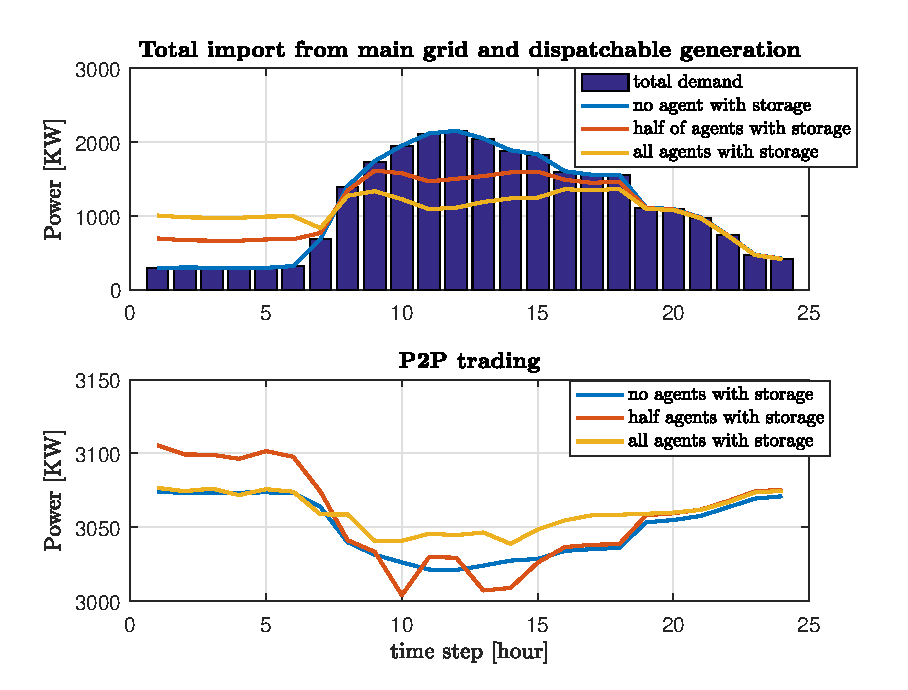
\includegraphics[width=1\linewidth]{simA_sto_37_3wtrade.eps}
        \caption{With trading among agents}
    \end{subfigure}%
    ~ 
    \begin{subfigure}{0.5\textwidth}
        \centering
        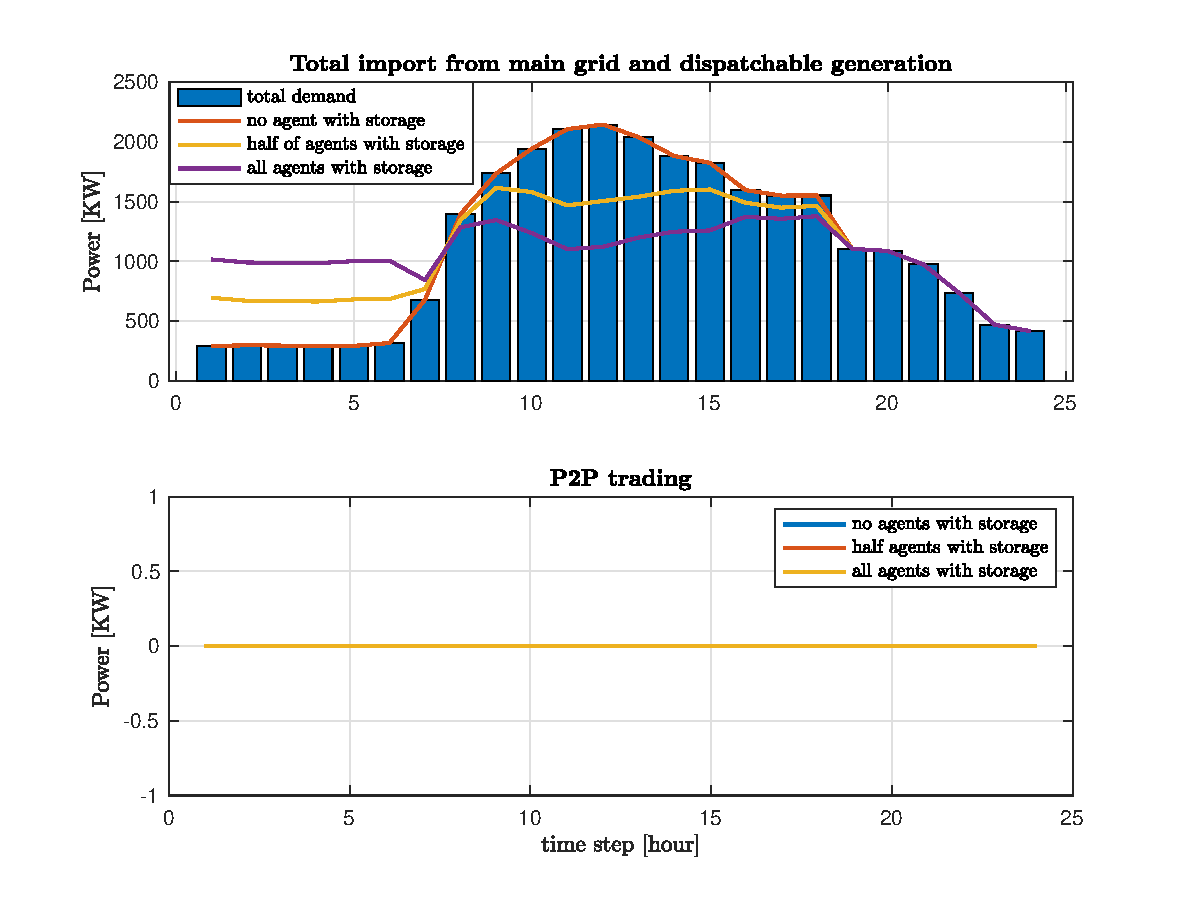
\includegraphics[width=1\linewidth]{simA_sto_37_3notrade.eps}
        \caption{Without trading among agents}
    \end{subfigure}
    \caption{Top: peak shaving effect of having storage units. Below: total trading among agents.}
    \label{fig:sim_A1}
\end{figure}
Top plots in \ref{fig:sim_A1}(a) and (b) do look very similar. I inspected closer, indeed total generations of dispatchable units between the case of with and without P2P trading are approximately the same. The differences may be caused by early termination of the algorithm since they are not large. Similarly, net powers imported from the main grid between the two cases are similar.  Note that in the case with trading, the ingoing power from the main grid is huge, but the outgoing is as well. The cost difference between the two cases of each group is also shown below in Figure 3. 
\begin{figure}[h]
	\centering
	\begin{subfigure}{0.5\textwidth}
		\centering
		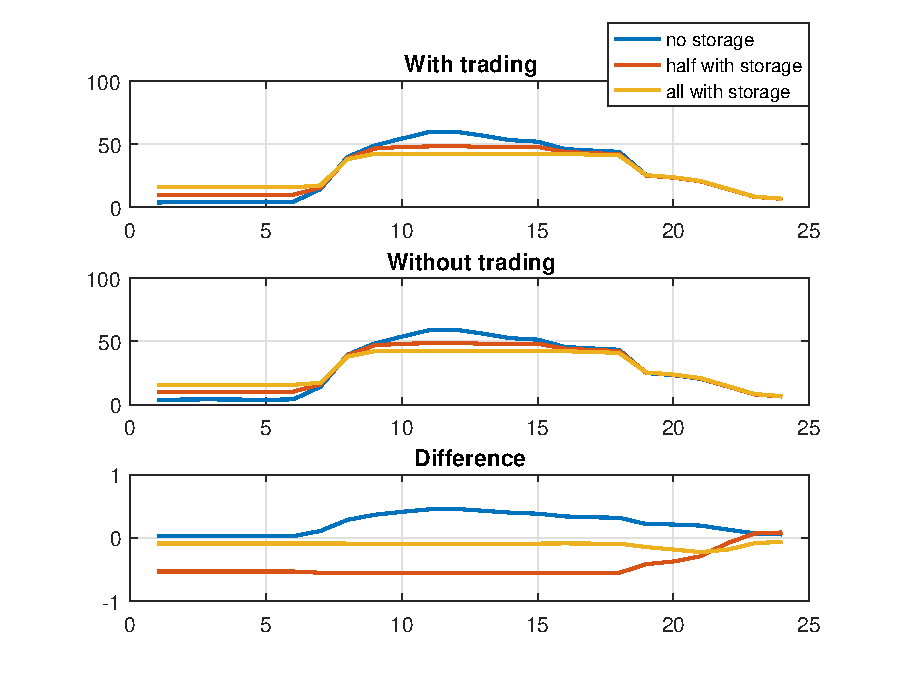
\includegraphics[width=1\linewidth]{pdi.eps}
		\caption{Total power generation by dispatchable units}
	\end{subfigure}%
	~ 
	\begin{subfigure}{0.5\textwidth}
		\centering
		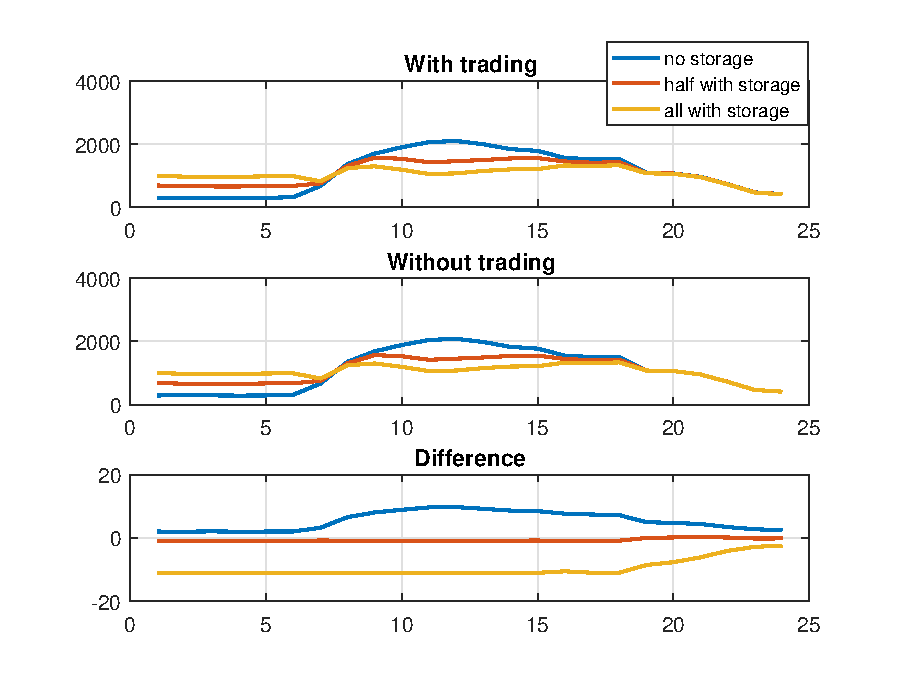
\includegraphics[width=1\linewidth]{pmg.eps}
		\caption{Net power imported from the main grid}
	\end{subfigure}
	%\caption{}
\end{figure}

\begin{figure}[h]
	\centering
	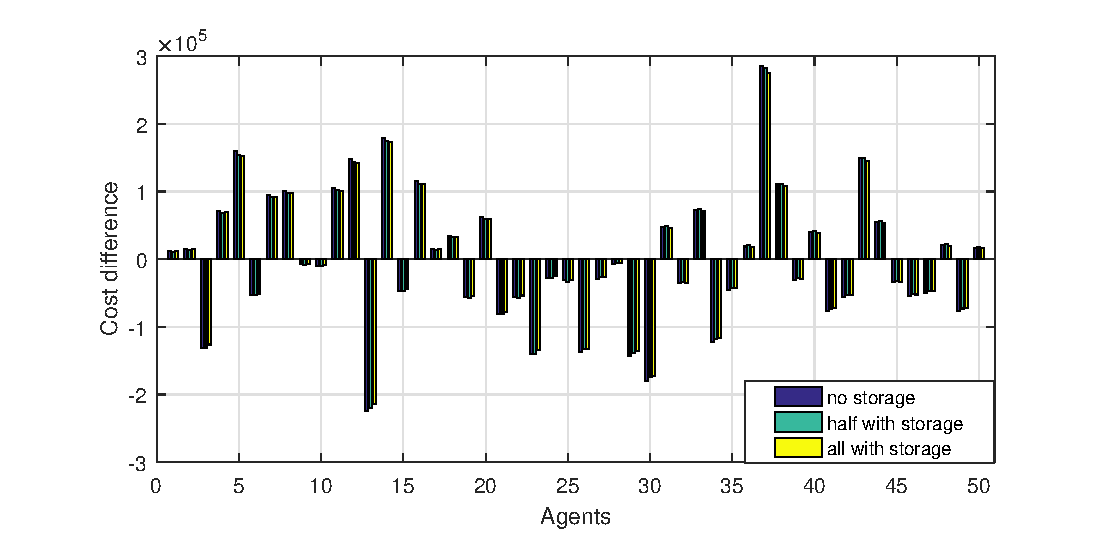
\includegraphics[width=1\linewidth]{simA_cost.eps}
	\caption{The cost difference between simulations without trading ($J_i$) and with trading ($J_i'$), i.e., $J_i-J_i'$, for each agent $i$.}
\end{figure}

%\newpage 
\section{Disallowing export power to the main grid}

\begin{figure}[h]
	\centering
	\begin{subfigure}{0.5\textwidth}
		\centering
		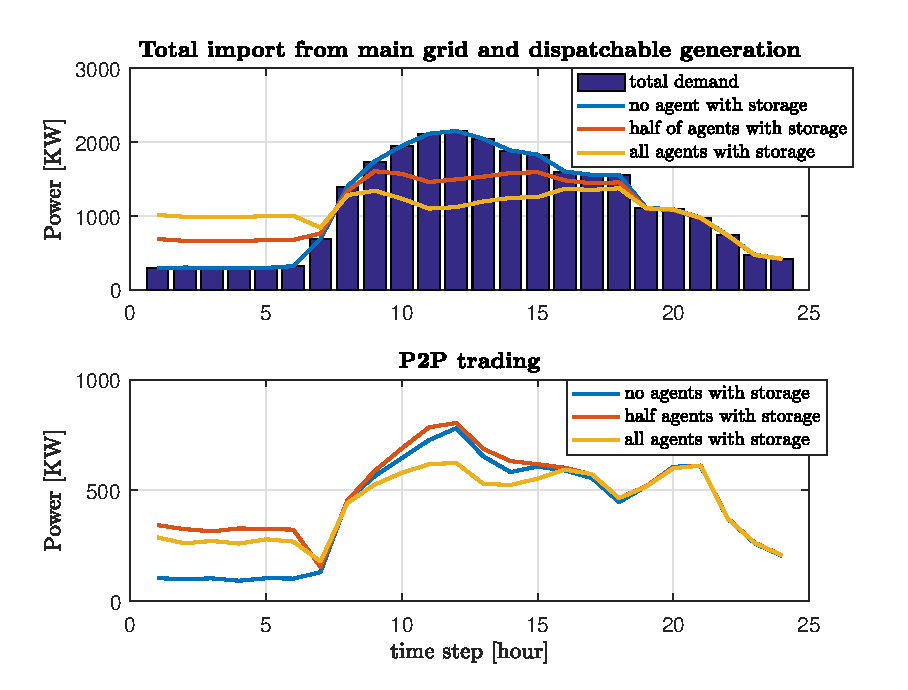
\includegraphics[width=1\linewidth]{simA_sto_37_4wtrade.eps}
		\caption{With trading among agents}
	\end{subfigure}%
	~ 
	\begin{subfigure}{0.5\textwidth}
		\centering
		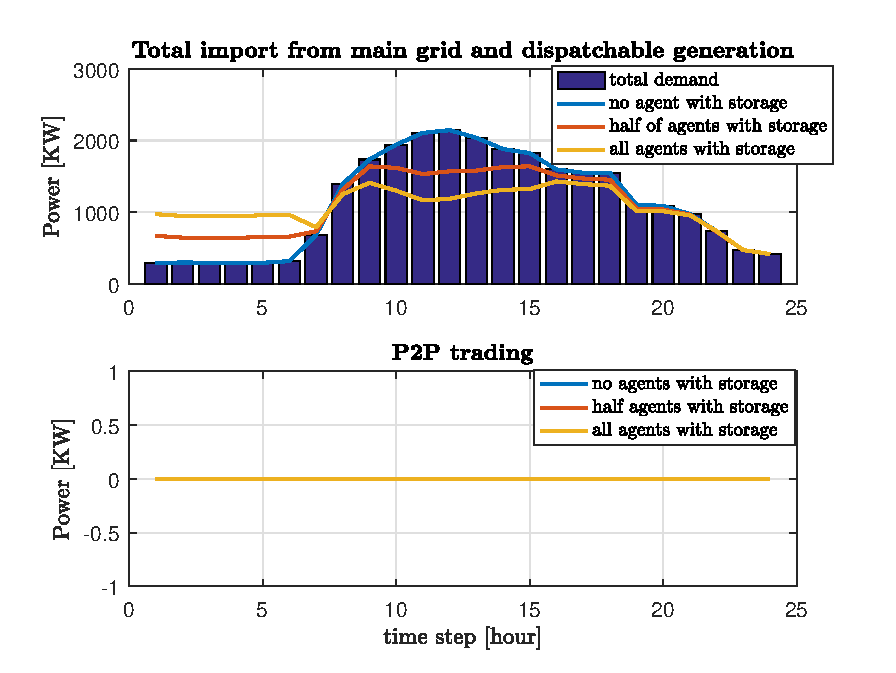
\includegraphics[width=1\linewidth]{simA_sto_37_4notrade.eps}
		\caption{Without trading among agents}
	\end{subfigure}
	\caption{(Disallowing export power to the main grid) Top: peak shaving effect of having storage units. Below: total trading among agents.}
	\label{fig:sim_A2}
\end{figure}

\begin{figure}[h]
	\centering
	\begin{subfigure}{0.5\textwidth}
		\centering
		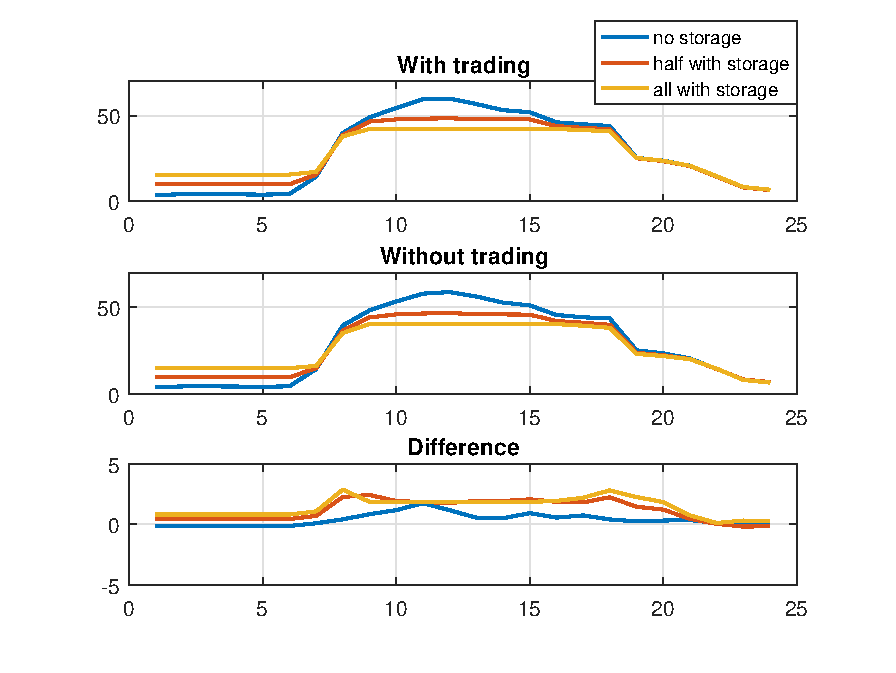
\includegraphics[width=1\linewidth]{pdi_2.eps}
		\caption{Total power generation by dispatchable units}
	\end{subfigure}%
	~ 
	\begin{subfigure}{0.5\textwidth}
		\centering
		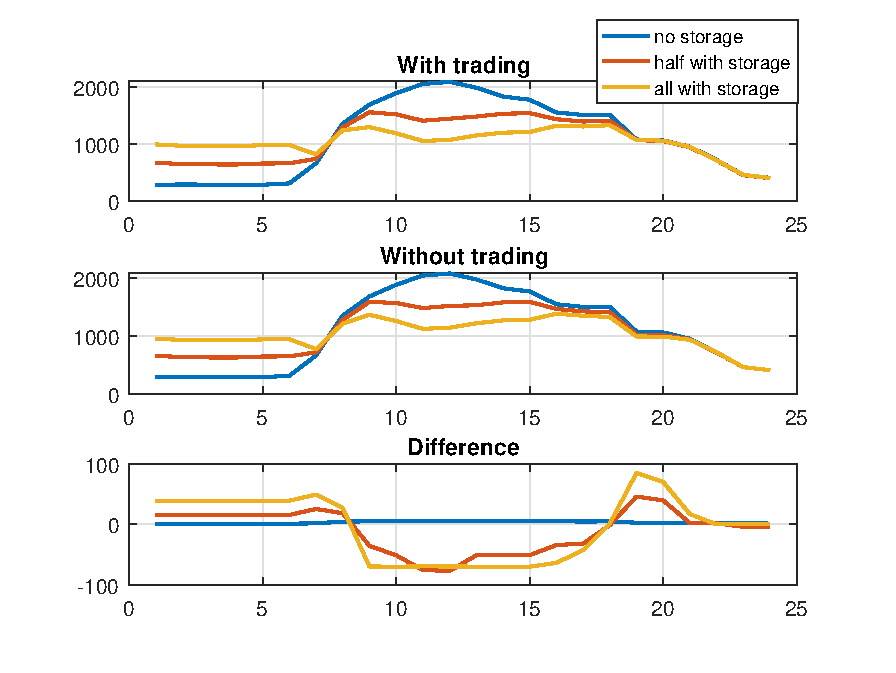
\includegraphics[width=1\linewidth]{pmg_2.eps}
		\caption{Net power imported from the main grid}
	\end{subfigure}
	\caption{(Disallowing export power to the main grid)}
\end{figure}


\begin{figure}[h]
	\centering
	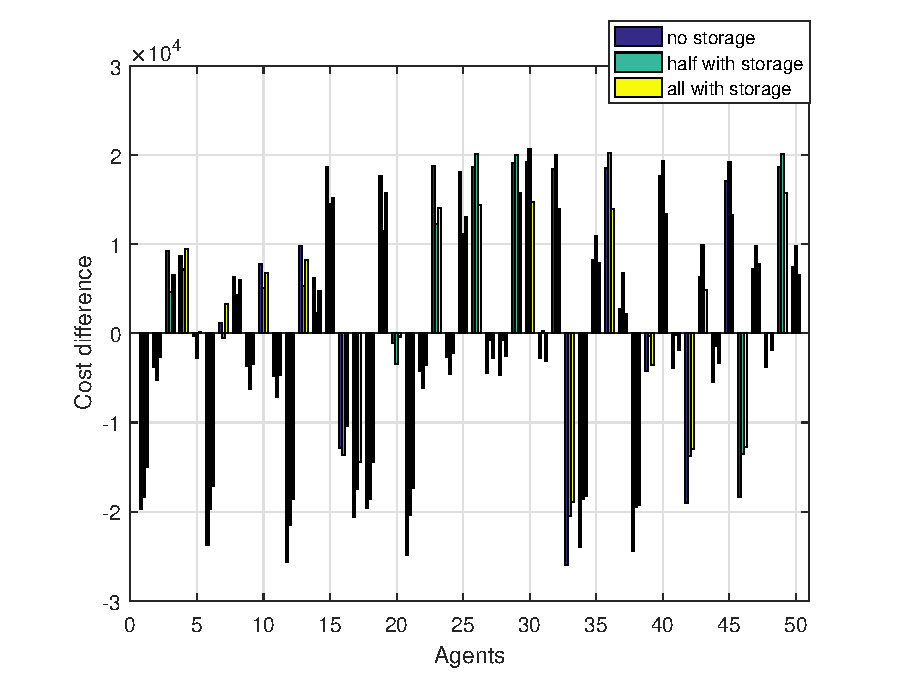
\includegraphics[width=1\linewidth]{simA_cost_2.eps}
	\caption{(Disallowing export power to the main grid) The cost difference between simulations without trading ($J_i$) and with trading ($J_i'$), i.e., $J_i-J_i'$, for each agent $i$. The differences of the total cost of the network $\sum_{i \in \mathcal N} (J_i-J_i')$:\\
		%\begin{itemize}
			- No storage: $-7\cdot10^3$.\\ 
			- Half with storage: $3.04\cdot 10^4$\\
			- All with storage: $2.23 \cdot 10^4$
		%\end{itemize}
	}
\end{figure}

%%%%%%%%%%%%%%%%%%%%%%%%%%%%%%%%%%%%%%%%%%%%%%%%%%%%%%
%\bibliographystyle{IEEEtran}
%\bibliography{IEEEfull,biblio}
%%%%%%%%%%%%%%%%%%%%%%%%%%%%%%%%%%%%%%%%%%%%%%%%%%%%%%
\end{document}

